\documentclass{article}
% Change "article" to "report" to get rid of page number on title page
\usepackage{amsmath,amsfonts,amsthm,amssymb}
\usepackage{setspace}
\usepackage{Tabbing}
\usepackage{fancyhdr}
\usepackage{lastpage}
\usepackage{extramarks}
\usepackage{url}
\usepackage{chngpage}
\usepackage{longtable}
\usepackage{soul,color}
\usepackage{graphicx,float,wrapfig}
\usepackage{enumitem}
\usepackage{morefloats}
\usepackage{multirow}
\usepackage{multicol}
\usepackage{indentfirst}
\usepackage{lscape}
\usepackage{pdflscape}
\usepackage{natbib}
\usepackage{algorithm}
\usepackage{algorithmic}
\usepackage[toc,page]{appendix}
\providecommand{\e}[1]{\ensuremath{\times 10^{#1} \times}}

% In case you need to adjust margins:
\topmargin=-0.45in      % used for overleaf
%\topmargin=0.25in      % used for mac
\evensidemargin=0in     %
\oddsidemargin=0in      %
\textwidth=6.5in        %
%\textheight=9.75in       % used for mac
\textheight=9.25in       % used for overleaf
\headsep=0.25in         %

% Homework Specific Information
\newcommand{\hmwkTitle}{Final Project Report}
\newcommand{\hmwkDueDate}{Friday,\ December\  7,\ 2018}
\newcommand{\hmwkClass}{Final Project}
\newcommand{\hmwkClassTime}{CSE 597}
\newcommand{\hmwkAuthorName}{Sahithi Rampalli}
\newcommand{\hmwkNames}{svr46}

% Setup the header and footer
\pagestyle{fancy}
\lhead{\hmwkNames}
\rhead{\hmwkClassTime: \hmwkTitle} 
\cfoot{Page\ \thepage\ of\ \pageref{LastPage}}
\renewcommand\headrulewidth{0.4pt}
\renewcommand\footrulewidth{0.4pt}

%%%%%%%%%%%%%%%%%%%%%%%%%%%%%%%%%%%%%%%%%%%%%%%%%%%%%%%%%%%%%
% Make title

\title{\vspace{2in}\textmd{\textbf{\hmwkClass}} \\
\vspace{0.1in}\large{ \hmwkClassTime}\vspace{3in}}

\author{\textbf{\hmwkAuthorName} \\ \vspace{0.1in}
\hmwkDueDate }
\date{} % to take away today's date

%%%%%%%%%%%%%%%%%%%%%%%%%%%%%%%%%%%%%%%%%%%%%%%%%%%%%%%%%%%%%

\begin{document}
\begin{spacing}{1.1}
\maketitle

\newpage
\section*{Abstract}



This final report on Conjugate Gradient solver for Discrete Poisson problem summarizes the various attempts to improve the performance of the solver on different platforms.
Initially, I implemented serial direct solver ($LDL^T$ transformation) and serial iterative solver (Conjugate Gradient) for solving Discrete Poisson problem on Cartesian grid. I analyzed the performance of iterative solver over direct solver and found that iterative solver has a considerable speedup. \\
Next, I profiled the serial iterative solver to identify the most compute intensive operations and found that matmul (stencil operation) is the major bottleneck. Then, I proposed ways to parallelize the iterative solver using OpenMP framework and obtained considerable speedup over the serial solver. I also analyzed how the performance varies by varying the number of cores and plotted the efficiency and speedup of the same (Strong Scaling). Finally, I execute Conjugate Gradient on GPU using OpenACC framework.  The results of this project will be used for our research work where we implemented conjugate gradient solver for the same problem on FPGA architecture \cite{FPGACG}. The aim is to compare the performance of the solver on different architectures including CPU, GPU and FPGA. Discrete Poisson Equation is used in various applications such as in computational fluid dynamics, theory of markov chains. A fast and efficient implementation of CG will be useful in accelerating many applications in the scientific community. In our research problem, we are trying to investigate various optimization techniques to come up with an efficient implementation of the solver which can be used in many scientific applications. It is more a mathematical problem than physical problem and we do not target a specific application.

In the following sections, I discuss the implementation and results of serial direct and iterative solver, parallel iterative solver on CPUs and GPUs. I also discuss other possible libraries that can be coupled with the iterative solver. 



\section{Problem of Interest}

    Finite difference numerical method is used to discretize the 2-dimensional Poisson equation. On an m{x}n grid, it takes the form
\[(\nabla^2	u)_{ij} = \dfrac{1}{dx^2}(u_{i+1,j} + u_{i-1,j} + u_{i,j+1} + u_{i,j-1} - 4u_{i,j} ) \] 
	Discrete Poisson equation arises in various fields of study such as heat flow, electrostatics, gravity, computational fluid dynamics, theory of markov chains and many more. They occur frequently in scientific computing, for instance, when solving partial diferential equations, in inexact newton methods for solving optimization problems in machine learning applications etc. The size of the grids on which the equation is applied can go as large as 10s or 100s of 1000s. For such large matrix sizes, it is clearly essential to parallelize and optimize the solvers. Hence, an efficient implementation of CG which can be used in various physical applications is necessary. For our research, we have not chosen a specific physical problem, but would like to contribute possible optimization techniques for this iterative solver. However, for the convergence test, we use a tolerance to control the number of iterations. \\
	Convergence criteria: I have chosen the tolerance to be of the order of $10^{-4}$ as this will ensure good accuracy for most applications involving discrete poisson equation. 
	The solver breaks when the logarithm of dot product of the residual values is greater than logarithm of the tolerance.
\[ delta = dotProduct(residual\_values); \epsilon = 0.0001 \]
\[ log_{10}(\sqrt{|delta|}) >= log_{10}(\epsilon) \] 
\\
	Since the matrix sizes are really large, direct solvers are usually not preferred as $A^{-1}$ computation or back filling will be quite expensive. Iterative methods like  Jacobi, SOR, Conjugate Gradients are used to solve discrete Poisson Equation \cite{Berkley1996}. Iterative methods use the idea of nearest-neighbour computation to solve the equation. SOR and CG take about the same number of steps. However, the advantage of CG over SOR is that CG can be used for larger class of problems. Methods like FFT and Multigrid can be faster than the iterative methods as they forward the information to points on the grid which are farther than the nearest neighbours. FFTs and multigrid are more specialized to solve problems like Poisson, unlike direct solvers like LU decomposition which is used to solve almost any linear system (non-singular). \cite{FFTPoisson}
	\\
	We have a simple MATLAB implementation of Conjugate Gradient. We used it to compare the accuracy of our FPGA implementation. I have also used it to compare the accuracy of direct solver, serial and parallel CG implementations. A pseudo code of CG is shown in algorithm \ref{algoCG}
	
\begin{algorithm}[H]

%\begin{multicols}{2}
\begin{algorithmic}[1]
%\caption{function [A, x, b] = CG(A, b)}

%\label{alg:seq}
\STATE $n = \text{size}(A,1)$ 
\STATE $x = \text{zeros}(n,1)$
%\STATE $resVec = [\hspace{1mm}]$
\STATE $r_{\text{old}} = b$ ; $p = r_{\text{old}}$ ; $j = 1$
\FOR{$i=1$ until convergence}
\STATE $z = A*p$ 
\STATE ${\alpha} = (r_{\text{old}}, r_{\text{old}})/(z, p)$
\STATE $x = x + \alpha * p$ 
\STATE $r = r_{old} - \alpha * z$
\STATE $\beta = (r, r) \, / \, (r_{\text{old}}, r_{\text{old}})$
\STATE $p = r + \beta* p$;
\STATE $r_{\text{old}} = r$
%\STATE $resVec = [resVec, norm(A * x - b)]$ 
%\STATE $j \gets j + 1$	
\ENDFOR
%\STATE $its = j$
\end{algorithmic}
%\end{multicols}
\caption{\label{algoCG} function [A, x, b] = stdCG(A, b)} 
\end{algorithm}

\subsection{Numerical Set-up}

\subsubsection{Direct Solver}
	I obtained the $A$ matrix for $LDL^T$ factorization using the MATLAB command "gallery('poisson', $n$)" where $n$ is the compute grid dimension which is half of the matrix dimension (say $N$). This MATLAB command generates the matrix based on the poisson equation discussed in section 1. The vector $b$ is populated with random numbers. As I am not focussing on a particular physical problem, using a random $b$ vector is meaningful. This would not affect the analysis or possible optimizations that we are investigating in any way. The same vector is used for both the solvers.

\subsubsection{Iterative Solver}
	For iterative solver, the matrix $A$ is not stored, but every matrix operation is visualized as a stencil operation computed on a grid of dimension $n$ which is half of the matrix dimension ($N$). The stencil operation is discussed in detail in the next section. The vector $b$ is same as that for direct solver.
\\
\newline
 The direct solver involves matrix vector multiplications. Without any optimizations, it is quite compute intesive to scale the problem to larger dimensions. Hence, for testing purposes, I chose matrix of sizes $64x64$, $256x256$ and $1024x1024$. The matrix dimensions for production problem can go upto 10s and 100s of 1000s. For our research work on FPGA, we used maximum matrix size of $10816x10816$. I claim that with multi-threading and matrix decomposition, the matrix dimension can go upto the order of $10^4$.
 \\
 For the applications of discrete poisson equation, the matrix dimensions can be of the order of $10^4$ or $10^5$. Due to the resource constraints (for storing larger matrices), I only use matrix dimensions upto order of $10^3$ to analyze the performance and then estimate the performance of serial solvers for larger dimension matrices.
\\
As mentioned, we are not targetting any particular physical problem. We mainly focus on the possible optimizations for the most compute intensive parts of the algorithms. Hence, we do not use any boundary conditions as they can be taken care during pre-processing or post-processing steps of the direct/iterative solver. For example, to solve the poisson's equation in an electrostatic setup, 
$\rho = \nabla^2\phi$,
for dirichlet boundaries $\phi(0) = D$, the condition can be implemented in the initial guess of the solution \cite{stackexchangeBoundary}. Hence, handling the boundary conditions is primarily dependent on the application.

\section{Solvers}

\subsection{Direct Solver}

As mentioned in the previous section, I use $LDL^T$ factorization as a direct solver for solving discrete poisson equation on large compute grids. An example of the poisson problem is shown in the figure \ref{poisson}.

\begin{center}
	\begin{figure}[H]
	\centering
       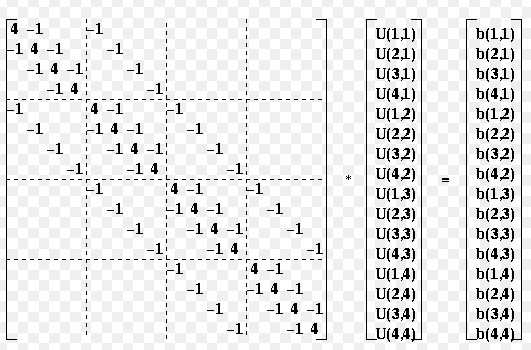
\includegraphics[scale=.40]{poisson.png}
        \caption{\label{poisson} Discrete Poisson Problem on 4x4 grid \cite{Berkley1996}.} 
	\end{figure}
\end{center}

Clearly the matrix can be viewed as a symmetric, banded matrix. When a matrix is symmetric, Cholesky decomposition ($LL^T$ factorization) is the optimal way to solve the linear system of equations. Since the above matrix is not only symmetric, but also diagonal dominated, a different version of Cholesky, $LDL^T$ factorization, is the best choice. 
If a matrix $A\epsilon R^{nxn}$ is symmetric and the principal submatrix $A(1:k,1:k)$ is nonsingular for $k=1:n-1$, then there exists a unit lower matrix $L$ and a diagonal matrix $D$ such that $LDL^T$ and the factorization is unique. \cite{MatComp}

The algorithm for $LDL^T$ factorization is shown in listing \eqref{algoLDL}. Here the matrix $A$ is overwritten with $D_i$ for $i=j$ and $L_{ij}$ for $i>j$.
\begin{algorithm}[H]

%\begin{multicols}{2}
\begin{algorithmic}[1]
%\caption{function [A, x, b] = LDLt(A, b)}

%\label{alg:seq}
\FOR{$j=1:n$}
\FOR{$i=1:j-1$ until convergence}
\STATE $v(i) = A(j,i)*A(i,i)$ 
\ENDFOR
\STATE $A(j,j) = A(j,j) - A(j,1:j-1).v(1:j-1)$
\STATE $A(j+1:n,j) = (A(j+1:n, j) - A(j+1:n,1:j-1).v(1:j-1))/A(j,j) $ 
%\STATE $resVec = [resVec, norm(A * x - b)]$ 
%\STATE $j \gets j + 1$	
\ENDFOR
%\STATE $its = j$
\end{algorithmic}
%\end{multicols}
\caption{\label{algoLDL} function [A, x, b] = $LDL^T(A, b)$} 
\end{algorithm}

The algorithm $LDL^T$ factorization requires about $n^3/3$ flops which is almost half the number of flops required for Gaussian Elimination. 

The implementation is also made memory-efficient by writing back to the matrix $A$ and vector $b$ and not using any other extra space. I also made an attempt to store $A$ as a banded matrix to reduce the space further. However, the logic did not work perfectly. I shall work on the logic and update the code in the coming days.

\subsubsection*{Timing and Memory}
For test problem, the chosen sizes of matrix A are $64x64$, $256x256$, $1024x1024$. The production problem size can be as large as $10861x10861$. 
The execution times for different test sizes upon using the G++ compiler optimization flag -O2 is shown in Table \ref{exec_direct}. The flag O2 has been chosen as it mainly optimizes for execution time and memory usage which are the important performance metrics I chose. I obtain similar performance with O3 flag and deproved performance with O1 flag. 
The memory required for matrix $A$ and vector $b$ is estimated in Kilobytes (KB). I obtained the virtual resident memory used by the task by executing the top unix command. 

\begin{table}[H]
\begin{center}
%\resizebox{\columnwidth}{!}{%
 \begin{tabular}{| c | c | c | c |} 
 \hline
$N$ & $Exec time (microseconds)$  & $Estimated Memory (KB)$ & $Memory (MB)$  \\ %[0.3ex] 
 \hline
64 & 758 & 16.25 & 2.42  \\ %\hline
256 &  18680 &257 & 3.11 \\ %\hline 
1024 &  1151817 & 4100 & 5.24 \\ %[0.3ex]
 \hline
\end{tabular}%
%}
\end{center}
\caption{\label{exec_direct} The execution time and number of elements stored for different test problem sizes.  } 
\end{table}

The execution time for back filling is shown in Table \ref{backfill_direct}.

\begin{table}[H]
\begin{center}
%\resizebox{\columnwidth}{!}{%
 \begin{tabular}{| c | c |} 
 \hline
$N$ & $Exec time (microseconds)$ \\ %[0.3ex] 
 \hline
64 & 74  \\ %\hline
256 &  372 \\ %\hline 
1024 &  10503  \\ %[0.3ex]
 \hline
\end{tabular}%
%}
\end{center}
\caption{\label{backfill_direct} The execution time for back filling for different test sizes.  } 
\end{table}

We can see that apart from the time for decomposition, the backfilling also takes considerable number of FLOPs and hence the execution time. 

The projection of execution time for production problem size $10816$x$10816$ is expected to be of the order of $10^8$ microseconds. The projection of memory for production problem size $10816$x$10816$ is estimated to be around 446.3 MB. Thus the space required grows exponentially with the problem size.


\subsection{Iterative Solver}

I use Conjugate Gradient (CG) method as an iterative solver for solving discrete poisson equation. One reason for choosing conjugate gradient is that it was developed for symmetric and positive definite matrices which is the case in the chosen problem. Also, as we are testing conjugate gradient on FPGA architecture, it would be useful to use this method and test it on CPU to compare the performance of our hardware design for CG with that on CPU.

Convergence criteria: I have chosen the tolerance to be of the order of $10^{-4}$. Most applications allow a tolerance upto order of $10^{-4}$ to $10^{-6}$. Even though I am not addressing a specific application, the choice of tolerance will not affect the trend in the performances of different matrix sizes as it will only increase the number of iterations. My inequality to test for convergence is:
\[ delta = dotProduct(residual_values); \epsilon = 0.0001 \]
\[ log_{10}(\sqrt{|delta|}) >= log_{10}(\epsilon) \]


\begin{algorithm}[H]

%\begin{multicols}{2}
\begin{algorithmic}[1]
%\caption{function [A, x, b] = CG(A, b)}

%\label{alg:seq}
\STATE $n = \text{size}(A,1)$ 
\STATE $x = \text{zeros}(n,1)$
%\STATE $resVec = [\hspace{1mm}]$
\STATE $r_{\text{old}} = b$ ; $p = r_{\text{old}}$ ; $j = 1$
\FOR{$i=1$ until convergence}
\STATE $z = A*p$ 
\STATE ${\alpha} = (r_{\text{old}}, r_{\text{old}})/(z, p)$
\STATE $x = x + \alpha * p$ 
\STATE $r = r_{old} - \alpha * z$
\STATE $\beta = (r, r) \, / \, (r_{\text{old}}, r_{\text{old}})$
\STATE $p = r + \beta* p$;
\STATE $r_{\text{old}} = r$
%\STATE $resVec = [resVec, norm(A * x - b)]$ 
%\STATE $j \gets j + 1$	
\ENDFOR
%\STATE $its = j$
\end{algorithmic}
%\end{multicols}
\caption{\label{algoCG} function [A, x, b] = stdCG(A, b)} 
\end{algorithm}

The Conjugate Gradient algorithm shown in \eqref{algoCG} has a matrix-vector multiplication operation $z=A*p$. However, one can view this operation as a stencil operation applied on the vector $p$. The stencil will be:
\begin{tabular}{|c|c|c|}
\hline
0 & -1 & 0\\ \hline
-1 & 4 & -1 \\ \hline
0 & -1 & 0 \\ \hline
\end{tabular}

This can be very easily deduced from the discrete poisson form shown in section 1.
Applying the stencil operation reduces the number of FLOPs exponentially as the stencil is computed on vector $p$ which is square root times the size of matrix $A$.
Performing $z=A*p$ as a stencil operation is not only compute-efficient but also memory-efficient as we do not have to store matrix $A$.

The convergence plot of $Log_{10}(Residual Values)$ Vs. $iterations$ is shown in the figure \ref{convPlot}. The plot is the same for all types of input initializations. I have tested the convergence of the solver for different and random input initializations including zero initialization and initialization based on a guess. Any type of initialization results in the same residuals values and hence the same convergence plot. (This has been tested multiple times.)
\begin{center}
	\begin{figure}[H]
	\centering
       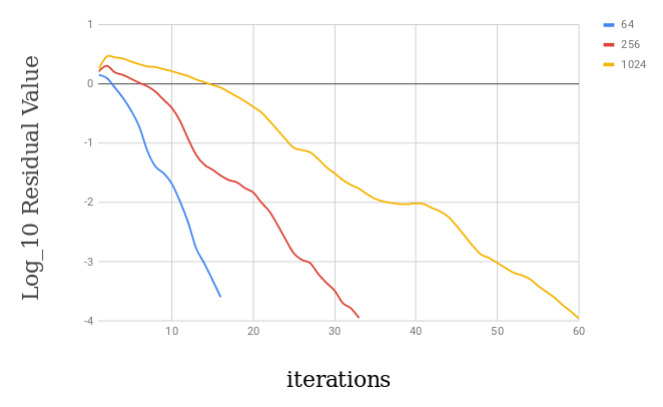
\includegraphics[scale=.40]{convergence.png}
        \caption{\label{convPlot} Convergence Plot} 
	\end{figure}
\end{center}


\subsubsection*{Timing and Memory}
For test problem, the chosen sizes of matrix $A$ are $64x64$, $256x256$, $1024x1024$. The production problem size can be as large as $10861x10861$. 
The execution times for different test sizes upon using the G++ compiler optimization flag -O2 is shown in Table \ref{exec_iter}. The flag O2 has been chosen as it mainly optimizes for execution time and memory usage which are the important performance metrics I chose. I obtain similar performance with O3 flag and deproved performance with O1 flag. Table \ref{exec_iter} also shows the estimated memory (in KB) and the memory required by the task (in MB). The memory estimation is based on the number of elements stored. 

I have tested the problem for different initializations for vector $x$. Any random initialization (tested multiple times) gives the same set of residual values and number of iterations. The possible reason is that the residual vector $r$ in conjugate gradient method is not much dependent on the values of $x$, which is evident from algorithm \eqref{algoCG}.

\begin{table}[H]
\begin{center}
%\resizebox{\columnwidth}{!}{%
 \begin{tabular}{| c | c|c|c|c|} 
 \hline
$N$ & $ExecTime (microseconds)$  & $Estimated Memory (KB)$ & $Memory (MB)$ \\ %[0.3ex] 
 \hline
64 & 155 &  1.25 & 0.97\\ %\hline
256 &  440 & 5 & 1.15\\ %\hline 
1024 &  4988 & 20 & 1.2\\ %[0.3ex]
 \hline
\end{tabular}%
%}
\end{center}
\caption{\label{exec_iter} The execution time and memory in KB for different test problem sizes.  } 
\end{table}

The size of the vector $b$ required for the problem increases linearly with the problem size.
The projection of execution time for production problem size $10816$x$10816$ is expected to be of the order of $10^6$ microseconds. The projection of memory for production problem size $10816$x$10816$ is expected to be around 212KB. Thus the space required grows linearly with the problem size. 


\subsection{Solver Comparison}
The table \ref{speedup} shows the speedup of the Conjugate Gradient method over the direct solver. Clearly, conjugate gradient method outperforms direct solver as the number of computations has reduced exponentially. Also, the speedup increases with increase in the matrix size.

From storage point of view, iterative solver wins over direct solver as the matrix $A$ is not stored in the former case (sparse matrix-vector multiplication operation is replaced by stencil operation). The number of elements required for CG increases linearly with problem size unlike the direct method where the growth is exponential.

Even for a production scale problem where matrix size is of the order $10^4$ and more, conjugate gradient will have greater speedup when compared to $LDL^T$ factorization.

It is clear that the execution time of direct solver, for production size problem is of the order of minutes which is pretty slow. Upon parallelizing the $LDL^T$ factorization, the matrix can be distributed among multiple threads for computation and the performance can be improved. Since, there may not be much communication/boundary sharing, the speedup due to parallelization can be close to the number of threads.

Also, for direct solver, the static memory allocation limits the size of the problem to be of the order $10^3$. As projeced in section 2.1, the memory requirement for production problem size is around 500MB which is too high for such applications. Nevertheless, the need for large space is eliminated in the iterative solver. For larger problems of order $10^5$ and higher, the memory required can be greater than 50MB and the processing time can be close to one minute. This can be improved by parallelizing the problem.

\begin{table}[H]
\begin{center}
%\resizebox{\columnwidth}{!}{%
 \begin{tabular}{| c | c |} 
 \hline
$N$ & $Exec time (microseconds)$  \\ %[0.3ex] 
 \hline
64 & 4.8x \\ %\hline
256 & 42.5x \\ %\hline 
1024 &  231x \\ %[0.3ex]
 \hline
\end{tabular}%
%}
\end{center}
\caption{\label{speedup} The speedup of CG over $LDL^T factorization$  } 
\end{table}


\section{Parallelization}

    The performance of the serial iterative solvers was discussed in detail in the previous report. There is a lot of scope for parallelization in CG as many operations are point-wise operations like dot-product of vectors, vector addition and subtraction. I chose to use OpenMP framework for parallelizing the CG as it is quite intuitive in the first observation that the operations can be easily distributed among multiple threads and can be accumulated at the end. Also, as taught in class, OpenMP framework has simple directives which leverage the implementation aspects and aptly portray the architecture we wish to realize. The matrix multiplication operation in line 5 of \ref{algoCG} is realized as a stencil operation applied on vector $p$ instead of a matrix multiplication operation. The stencil will be:
\begin{tabular}{|c|c|c|}
\hline
0 & -1 & 0\\ \hline
-1 & 4 & -1 \\ \hline
0 & -1 & 0 \\ \hline
\end{tabular}

This can be very easily deduced from the discrete poisson form shown in section 1.  This stencil operation can also be parallelized using OpenMP.
    \\
    pthread Library: We can use the pthread library of C/C++ to accomplish the same. In fact, OpenMP directives can be directly mapped to the pthread functions. However, from programming point of you, OpenMP is simple and easy to use and keeps the code less complex.
    \\
    \\
    MPI: I propose a parallelization technique on stencil operation using MPI. Please note that the stencil operation is the first operation performed in every iteration of CG. We can scatter the vector, on which stencil is applied, among multiple cores using MPI\_SCATTER   and gather the final result after the operation using MPI\_GATHER. This can be applied to all other operations in CG. However, the OpenMP implementation is almost equivalent to this idea.  Hence, I have not evaluated/analyzed the CG implementation using MPI.
    \\
    \\
    MapReduce: In section 3.2, I discuss an alternative approach to parallelize CG. Though I have not used the MapReduce framework, I implemented an equivalent way to parallelize the stencil operation. In this approach, I divide the computation grid on which the stencil is applied, into 4 blocks (for 4 threads), perform stencil operation parallely on individual blocks and then accumulate the result into a shared grid. A similar idea is applicable for rest of the vector operations - dot product, vector addition and subtraction. Due to the simplicity and directness of OpenMP, I used that framework. 
    \\
    \\
    PGAS: As I have used C++ to implement the direct and iterative solvers for Project Report #1, I started with applying simple OpenMP directives to the existing code to identify which parts of the code can be parallelized. Later, I did not switch to a new language PGAS. PGAS is relavant to my implementation and partially shares the same idea as my implementation.
    
   
    The simple point-wise operations - dot product, vector addition and subtraction - can be applied on part of the vectors by individual threads. No thread communication is required for these point-wise operations. This can be achieved using simple directives in OpenMP. It is worth nothing that the result of the dot product operation has to accumulated in a single shared variable. This can be achieved by accumulating the result of each thread (applied on a part of the vector) in a private variable which can be added to the shared variable in a critical section. However, using the OpenMP directive, "reduction(+: shared variable)" also serves the purpose. 
 \\
        The stencil operation can also be parallelized. The threads can be scheduled statically on this operation. All threads apply stencil operations on different elements parallely. 
    
        All the major operations of each iteration are parallelized except for a few operations such as computing the alpha and beta in lines 6 and 9 of algorithm \ref{algoCG} respectively and computing the distance from tolerance after every iteration, which are critical sections of the code and need to be performed only by a single thread. 
        The percentage of parallel sections for different matrix dimensions is shown in table \ref{percent}.
\begin{table}[H]
\begin{center}
%\resizebox{\columnwidth}{!}{%
 \begin{tabular}{| c | c|} 
 \hline
Matrix dimension & Percentage of Parallel Code  \\ %[0.3ex] 
 \hline
1024 & 78.26 \\ %\hline
1600 &  73.6\\ %\hline 
10816 &  88.7\\ %[0.3ex]
 \hline
\end{tabular}%
%}
\end{center}
\caption{\label{percent} Percentage of Parallel Code.   } 
\end{table}

    
     There is no difference in the numerical setup for the iterative solver. The matrix $A$ is not stored, but every matrix operation is visualized as a stencil operation computed on a grid of dimension $n$ which is half of the matrix dimension ($N$). The vector $b$ is randomly generated. 
     The sample matrix sizes considered are $1024x1024$, $1600x1600$ and $10816x10816$. 
     The production matrix sizes are $250000x250000$ and $1000000x1000000$.
     For weak scaling, different set of sample matrix sizes were used as the ratio of number of cores to problem sizes have to remain constant. \\
     As mentioned in project report #1, the convergence of CG did not vary with change in the initialization of $x$. Hence, I considered the case where $x$ is initialized to zero. \\

\subsection{Profiling}

\subsubsection{Serial}
The tables  \ref{serial1024}, \ref{serial1600}, \ref{serial10816} show the profiles of the serial CG code for sample matrix dimensions 1024, 1600 and 10816 respectively. As expected, the Matmul (stencil operation) takes maximum percentage of time for any matrix dimension as the number of operations in this function are more than that in any other vector operation functions. 5 Operations are performed on each grid element as can be seen in the discrete Poisson equation in section 1. 

\begin{table}[H]
\begin{center}
%\resizebox{\columnwidth}{!}{%
 \begin{tabular}{| c | c|c|c|} 
 \hline
$Name$ & $Exclusive Time (msec)$ & $\% Time$ & $#Call$  \\ %[0.3ex] 
 \hline
Matmul & 0.788 & 12.2& 61\\ %\hline
VectorAdd1 &  0.296& 4.6 & 61\\ %\hline 
VectorAdd2 &  0.291& 4.5 & 61\\ %[0.3ex]
VectorSub &  0.295& 4.6 & 61\\ %[0.3ex]
DotProduct1 &  0.238& 3.7 & 61\\ %[0.3ex]
DotProduct2 &  0.239& 3.7& 61\\ %[0.3ex]
 \hline
\end{tabular}%
%}
\end{center}
\caption{\label{serial1024} Profile of Serial code for matrix size: 1024   } 
\end{table}

\begin{table}[H]
\begin{center}
%\resizebox{\columnwidth}{!}{%
 \begin{tabular}{| c | c|c|c|} 
 \hline
$Name$ & $Exclusive Time (msec)$ & $\% Time$ & $#Call$  \\ %[0.3ex] 
 \hline
Matmul & 1 & 17.9 & 82\\ %\hline
VectorAdd1 &  0.608 &6.7 & 82\\ %\hline 
VectorAdd2 &  0.596 & 6.5 & 82\\ %[0.3ex]
VectorSub &  0.606 & 6.6 & 82\\ %[0.3ex]
DotProduct1 &  0.487 & 5.3 & 82\\ %[0.3ex]
DotProduct2 &  0.488 & 5.3 & 82\\ %[0.3ex]
 \hline
\end{tabular}%
%}
\end{center}
\caption{\label{serial1600} Profile of Serial code for matrix size: 1600  } 
\end{table}

\begin{table}[H]
\begin{center}
%\resizebox{\columnwidth}{!}{%
 \begin{tabular}{| c | c|c|c|} 
 \hline
$Name$ & $Exclusive Time (msec)$ & $\% Time$ & $#Call$  \\ %[0.3ex] 
 \hline
Matmul & 26& 33.6 & 198\\ %\hline
VectorAdd1 &  9 &11.9 & 198\\ %\hline 
VectorAdd2 &  9 & 11.8 & 198\\ %[0.3ex]
VectorSub &  9& 12.1 & 198\\ %[0.3ex]
DotProduct1 &  7 & 9.5 & 198\\ %[0.3ex]
DotProduct2 &  7 & 9.5 & 198\\ %[0.3ex]
 \hline
\end{tabular}%
%}
\end{center}
\caption{\label{serial10816} Profile of Serial code for matrix size: 10816   } 
\end{table}


\\
Hence, I would like to focus on Matmul, the bottleneck, to improve performance. In order to perform the stencil operation, I currently use multiple conditional statements to check for boundary conditions while applying a stencil operation. An alternative way to perform stencil operation is to pad the given matrix with zeros on all sides and smoothly apply the stencil operation on the entire matrix. I implemented this alternative way and the profiles of the alternative serial CG code are shown in tables \ref{pad1024}, \ref{pad1600}, \ref{pad10816}. It can be seen that the Execution time of Matmul operation reduced for a given matrix size when padding is used. However, an extra function for padding has to be used. The aggregate time for execution of Matmul and Pad function is almost comparable to the previous Matmul function with conditional statements.

\begin{table}[H]
\begin{center}
%\resizebox{\columnwidth}{!}{%
 \begin{tabular}{| c | c|c|c|} 
 \hline
$Name$ & $Exclusive Time (msec)$ & $\% Time$ & $#Call$  \\ %[0.3ex] 
 \hline
Matmul & 0.506 & 8.3& 61\\ %\hline
PadFunction & 0.215 & 3.5& 61\\ %\hline

 \hline
\end{tabular}%
%}
\end{center}
\caption{\label{pad1024} Profile of Padded Serial code for matrix size: 1024   } 
\end{table}

\begin{table}[H]
\begin{center}
%\resizebox{\columnwidth}{!}{%
 \begin{tabular}{| c | c|c|c|} 
 \hline
$Name$ & $Exclusive Time (msec)$ & $\% Time$ & $#Call$  \\ %[0.3ex] 
 \hline
Matmul & 1 & 12.5 & 82\\ %\hline
PadFunction & 0.215 & 5.4& 82\\ %\hline
 \hline
\end{tabular}%
%}
\end{center}
\caption{\label{pad1600} Profile of Padded Serial code for matrix size: 1600  } 
\end{table}

\begin{table}[H]
\begin{center}
%\resizebox{\columnwidth}{!}{%
 \begin{tabular}{| c | c|c|c|} 
 \hline
$Name$ & $Exclusive Time (msec)$ & $\% Time$ & $#Call$  \\ %[0.3ex] 
 \hline
Matmul & 17& 22.7 & 198\\ %\hline
PadFunction & 7& 9.6 & 198\\ %\hline
 \hline
\end{tabular}%
%}
\end{center}
\caption{\label{pad10816} Profile of Padded Serial code for matrix size: 10816   } 
\end{table}

\\
I propose another technique to implement the stencil operation. The notion is to have some kind of pipeline design in Matmul. In this design, we use line buffers of size $3xGRID\_ COLUMN\_SIZE$ to cache every three rows of the grid. Note that, grid is the 2D vector representation on which the stencil is applied. The number three is chosen as the stencil dimension is three. Every element passes through the following pipeline stages.
\begin{itemize}
    \item The new element is updated in the line buffer.
    \item A current pointer is maintained to represent the locations on the line buffer where stencil is to be applied.
    \item The current pointer is used to update a window buffer of size $3x3$ (size of the stencil) which is the buffer on which stencil is applied.
    \item Finally, the stencil is applied on the window buffer.
\end{itemize}
We have used a similar pipelined approach in our FPGA implementation of CG. Please refer to the section III-B of \cite{FPGACG} for a better explanation. However, I have not included the evaluation of this method in the report.


\subsubsection{Parallel}

The profiles of parallel CG code for sample matrix sizes 1024, 1600 and 10816 using 4 threads are shown in tables \ref{ll1024}, \ref{ll1600}, \ref{ll10816} respectively. The Exclusive Time shown is mean of the exclusive time of each thread in a function. It can be seen that Matmul still takes the maximum amount of time among all functions. This is expected as the number of operations are split equally among all threads in any function. The total number of operations per thread has reduced. However, the number of operations in Matmul is still greater than that in other functions for a given thread. I have used static scheduling during parallelization as all threads perform similar operation. 

\begin{table}[H]
\begin{center}
%\resizebox{\columnwidth}{!}{%
 \begin{tabular}{| c | c|} 
 \hline
$Name$ & $Mean Exclusive Time (msec)$   \\ %[0.3ex] 
 \hline
Matmul & 0.26 \\ %\hline
VectorAdd1 &  0.148 \\ %\hline 
VectorAdd2 &  0.15\\ %[0.3ex]
VectorSub &  0.148\\ %[0.3ex]
DotProduct1 &  0.127\\ %[0.3ex]
DotProduct2 &  0.131\\ %[0.3ex]
 \hline
\end{tabular}%
%}
\end{center}
\caption{\label{ll1024} Mean Exclusive Time in msec of Parallel code for matrix size: 1024 using 4 threads. } 
\end{table}

\begin{table}[H]
\begin{center}
%\resizebox{\columnwidth}{!}{%
 \begin{tabular}{| c | c|} 
 \hline
$Name$ & $Mean Exclusive Time (msec)$   \\ %[0.3ex] 
 \hline
Matmul & 0.476 \\ %\hline
VectorAdd1 &  0.267 \\ %\hline 
VectorAdd2 &  0.278\\ %[0.3ex]
VectorSub &  0.258\\ %[0.3ex]
DotProduct1 &  0.224\\ %[0.3ex]
DotProduct2 &  0.22\\ %[0.3ex]
 \hline
\end{tabular}%
%}
\end{center}
\caption{\label{ll1600} Mean Exclusive Time in msec of Parallel code for matrix size: 1600 using 4 threads. } 
\end{table}

\begin{table}[H]
\begin{center}
%\resizebox{\columnwidth}{!}{%
 \begin{tabular}{| c | c|} 
 \hline
$Name$ & $Mean Exclusive Time (msec)$   \\ %[0.3ex] 
 \hline
Matmul & 6 \\ %\hline
VectorAdd1 &  3 \\ %\hline 
VectorAdd2 &  3\\ %[0.3ex]
VectorSub &  3\\ %[0.3ex]
DotProduct1 &  2\\ %[0.3ex]
DotProduct2 &  2\\ %[0.3ex]
 \hline
\end{tabular}%
%}
\end{center}
\caption{\label{ll10816} Mean Exclusive Time in msec of Parallel code for matrix size: 10816 using 4 threads. } 
\end{table}

The speedup of the parallel code over serial code for all sample matrix sizes is shown in table \ref{compspedup}. It can be noticed that parallel code is performing better than serial code for all sample matrix sizes. Also, the speedup is increasing with the increase in matrix dimensions. This is because for smaller matrix sizes, the communication overhead dominates the thread level parallelism which is compensated in case of larger matrices.
\begin{table}[H]
\begin{center}
%\resizebox{\columnwidth}{!}{%
 \begin{tabular}{| c | c|c|c|} 
 \hline
$Name$ & Speedup (N=1024) & Speedup (N=1600) & Speedup (N=10816)    \\ %[0.3ex] 
 \hline
Matmul & 3.03 &  2.1 & 4.33 \\ %\hline
VectorAdd1 &  2  &2.27   & 3 \\ %\hline 
VectorAdd2 &  1.94 &  2.14 &3 \\ %[0.3ex]
VectorSub &  1.99 &  2.35 & 3\\ %[0.3ex]
DotProduct1 &  1.87 &  2.17 &3.5 \\ %[0.3ex]
DotProduct2 &  1.82 &  2.22 & 3.5\\ %[0.3ex]
 \hline
\end{tabular}%
%}
\end{center}
\caption{\label{compspedup} Speedup of parallel code over serial code for sample matrix sizes.} 
\end{table}
\\
The table shows the time and memory estimates for production size matrix dimensions 250000 and 1000000, when run on 12 threads. The memory usage is obtained using the 'top' unix command.
\begin{table}[H]
\begin{center}
%\resizebox{\columnwidth}{!}{%
 \begin{tabular}{| c | c|c|} 
 \hline
 N & Exec Time (sec) & Memory (MB)   \\ %[0.3ex] 
 \hline
250000 & 0.8 & 29.3 \\ %\hline
1000000 & 6.6  & 69.3 \\ %\hline 

 \hline
\end{tabular}%
%}
\end{center}
\caption{\label{compspedup} Estimate of execution time and memory for production matrix dimensions when run on 12 threads.} 
\end{table}

As Matmul is taking maximum percentage of time. I tried to optimize this function. The stencil operation can also be parallelized by partitioning the computation grid such that the stencil operation is applied on each partition by individual threads (called Partitioned Parallel Code). I partitioned the grid into 4 blocks, each to be executed by a thread. Each block shares a row a neighbouring block and a column with a neighbouring block. The data of each partition is copied to a private data structure of each thread (called Copy Partial Data). The boundary data is copied to private buffers of each thread (called Copy Boundary Data).  Hence, the stencil operation is applied on individual blocks (called Partial Matmul). After the operation is performed, all threads write their outputs to a shared data structure (called Accumulate Output). The idea behind this modification is to investigate whether having private data structures for each thread will lead to better performance as the private data structures will be stored in the private caches of each cores. In the previous case, OpenMP directive was used to assign tasks to each thread to be performed on a shared memory. Though the number of stencil operations is same in both the cases, I wanted to investigate if manually partitioning the data will be more advantageous than having a shared data structure.  Table \ref{partition} shows the profile of the modified stencil operation. Though the partial Matmul operation performs better than the usual Matmul, the aggregate of Partial Matmul, pre-processing and post-processing is worse than Matmul for all matrix sizes.


\begin{table}[H]
\begin{center}
%\resizebox{\columnwidth}{!}{%
 \begin{tabular}{| c | c|c|c|} 
 \hline
$Name$ & Mean Time msec (1024) & Mean Time msec (1600) & Mean Time msec (10816)    \\ %[0.3ex]
 \hline
Partial Matmul & 0.147 &  0.297 & 4.26 \\ %\hline
Copy Partial Data & 0.117 &  0.188 & 2.43 \\ %\hline
Copy Boundary Data & 0.0253 & 0.036 & 0.146 \\ %\hline
Accumulate Output & 0.12 &  0.17 & 1.827 \\ %\hline
\cline{2-4}
Aggregate & 0.4093& 0.695 & 8.67\\%\hline
 \hline
\end{tabular}%
%}
\end{center}
\caption{\label{partition} Mean Time in msec of Partitioned Parallel code for matrix sizes 1024, 1600 and 10816. } 
\end{table}
\\



\subsection{Scaling}
In order to compute the strong scaling efficiency, I used 20 cores of Intel IvyBridge compute node, computed the the execution times of each problem size with varying number of cores from 1 to 20 (called \#Cores). Finally, efficiency of $x$ number of cores is computed as Speedup of $x$ number of cores over 1 core, averaged over $\#Cores$.
The plot of efficiency of parallel code for matrix sizes 1600 and 10816, for 20 cores, is shown in figure \ref{eff}. It can be seen that the efficiency decreases with the increase in number of cores. Single core has the maximum efficiency. Also, the efficiency is better for large matrix size as more percentage of resources are used in case of large matrix sizes. 


\begin{center}
	\begin{figure}[H]
	\centering
       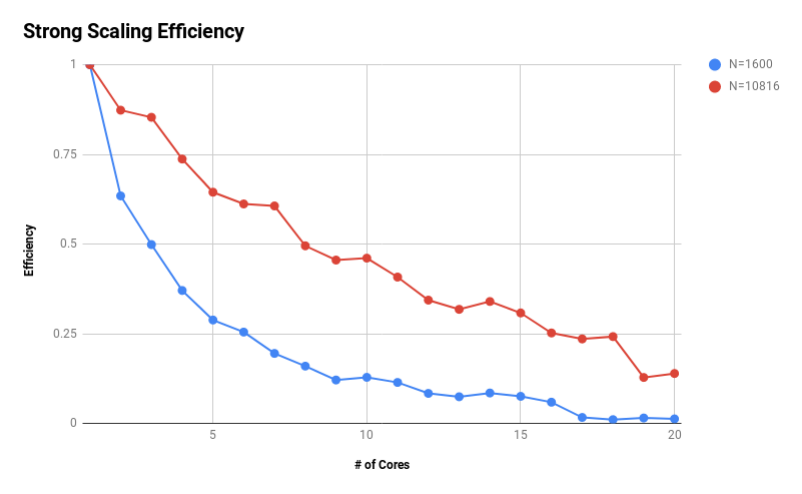
\includegraphics[scale=.40]{strongscaling.png}
        \caption{\label{eff} Efficiency of parallel code for matrix sizes 1600 and 10816.} 
	\end{figure}
\end{center}

Figure \ref{Speedup} shows the speedup of parallel code for matrix sizes 1600 and 10816 for 20 cores. The speedup decreases rapidly beyond certain number of cores. This is because of communication overhead among cores and the thread handling (creation, joining etc) is higher for more number of cores and it dominates the parallelism. It can be seen that the speedup for larger matrix is more than that for smaller matrix. This is because the communication overhead is amortized over the matrix size. 

\begin{center}
	\begin{figure}[H]
	\centering
       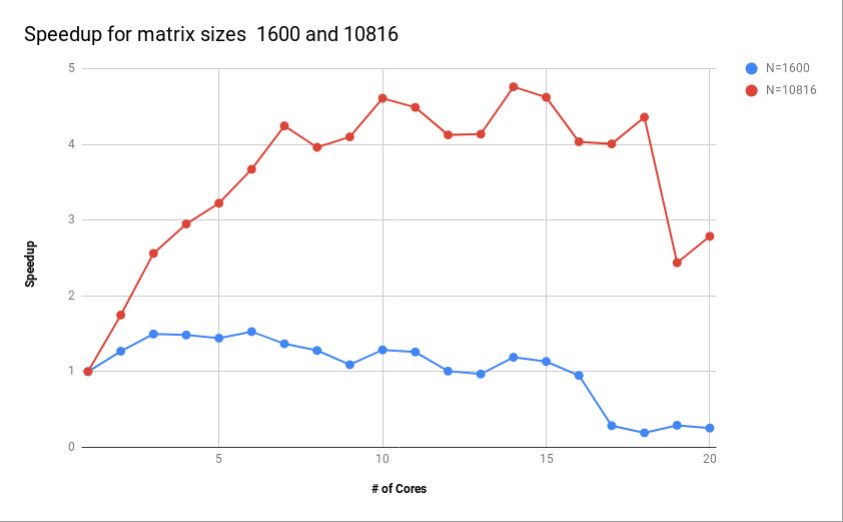
\includegraphics[scale=.40]{speedup_pr2.png}
        \caption{\label{Speedup} Speedup of parallel code for matrix sizes 1600 and 10816.} 
	\end{figure}
\end{center}


\begin{itemize}
    \item If speed is the concern, 6 and 14 cores would be best suitable for problems of size 1600 and 10816 respectively. 
    \item For perfectly efficient use of resources, single core would give the best results for any matrix size.
    \item For our research purposes, I would choose a reasonably efficient problem with close to maximum speedup. Speedup is more important for my case. Thus, 3 cores would be appropriate for matrix size 1600 and 10 cores would be appropriate for matrix size 10816. The efficiency for both are close to 0.5.
\end{itemize}
Thus, the optimal starting point for problem sizes greater than or equal to 10816 would be 10 cores. \\
\\
The plots \ref{Speedup1600} and \ref{Speedup10816} show the speedup of parallel code for matrix sizes 1600 and 10816 along with the theoretical speedup given by Amdahl's law and the ideal speedup which is equal to the number of cores used. The percentage of parallel code for matrix sizes 1600 and 10816 are 73.6\%  and 88.7\% respectively. As the matrix size increases, the speedup is closer to the theoretical speedup from Amdahl's law for more number of cores. In case of matrix size 1600, the obtained speedup is close to the theoretical speedup upto 2 cores. In case of matrix size 10816, the obtained speedup is close to the theoretical speedup upto 10 cores. \\
In the plot of speedup for matrix 10816, the curve has multiple local minima. A decrease in speedup beyond certain number of cores is expected as the communication overhead could be more dominant than the parallelism effect. However, we can find some local minima even for smaller number of cores. For instance, the speedup for 8 and 9 cores is less than that for 10 cores. The reason could probably be that the matrix dimension is not an exact multiple of number of cores and the code uses static scheduling. Hence, all cores may not finish at the same time and some cores have to wait for the rest of the cores to finish wherever there is a barrier.

\begin{center}
	\begin{figure}[H]
	\centering
       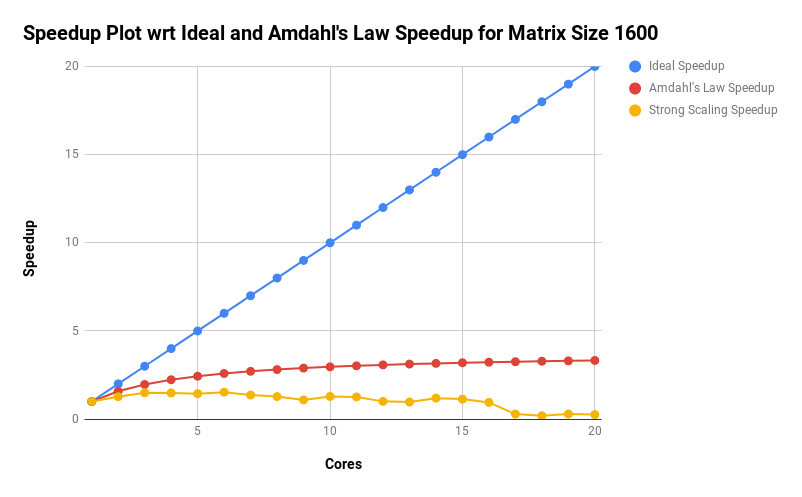
\includegraphics[scale=.40]{speedup1600_pr2.png}
        \caption{\label{Speedup1600} Speedup of parallel code for matrix size 1600 along with theoretical speedup given by Amdahl's law and the ideal speedup.} 
	\end{figure}
\end{center}

\begin{center}
	\begin{figure}[H]
	\centering
       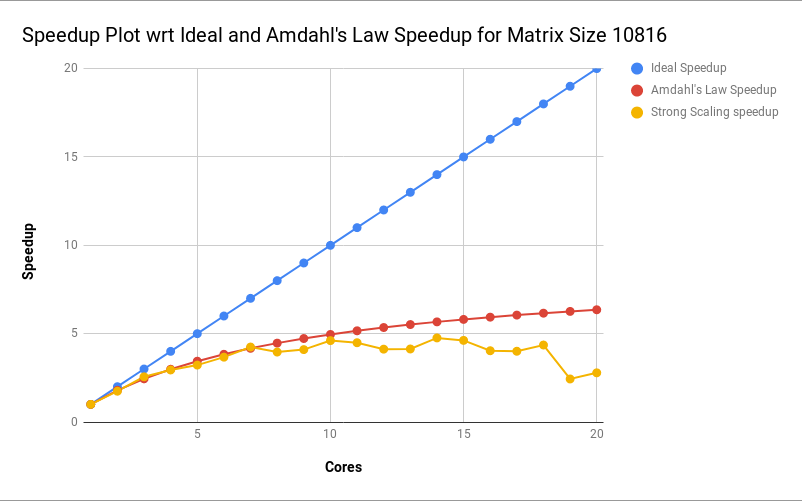
\includegraphics[scale=.40]{speedup10816_pr2.png}
        \caption{\label{Speedup10816} Speedup of parallel code for matrix size 160816 along with theoretical speedup given by Amdahl's law and the ideal speedup..} 
	\end{figure}
\end{center}

\subsection{Weak Scaling}
The weak scaling efficiency is computed as speedup of $x$ number of cores over 1 core. 
The Weak scaling efficiency plot is shown in figure \ref{weakscaling}. The horizontal axis represents the tuple (cores, matrix size). The matrix sizes here are different as the ratio of cores and matrix size has to remain constant in the plot. Clearly, the efficiency decreases with the increase in number of cores used and hence, the matrix size.


\begin{center}
	\begin{figure}[H]
	\centering
       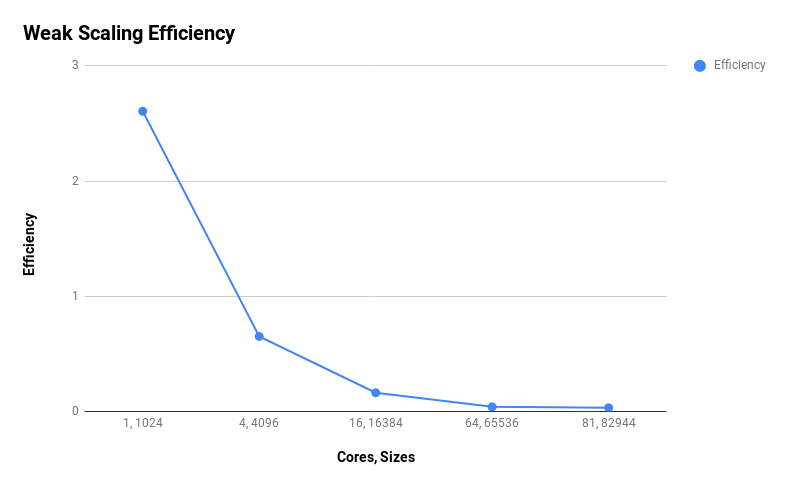
\includegraphics[scale=.40]{weakscaling.png}
        \caption{\label{weakscaling} Weak Scaling Efficiency plot .} 
	\end{figure}
\end{center}

\section{Coupling to an External Library}

\subsection{Coupling}

    As can be seen from table \ref{compspedup}, we achieved a good speedup for all test matrix sizes by parallelizing the code using 4 threads in OpenMP framework. Plot \ref{Speedup} showed the speedup with different number of cores. In order to further improve the performance over the OpenMP code, I decided to run CG on GPUs. I expect a better speedup with GPUs as most of the operations in CG are SIMD operations (dot product, vector additions/subtractions and stencil operation). I believe dividing these SIMD operations among manycore GPUs will greatly enhance the speedup. I ran all the functions/major operations of CG on GPU. The different operations can be seen in table \ref{gpu_profile}\\
    I am using OpenACC framework to parallelize CG for GPUs and execute it. 
    OpenACC has pragmas similar to OpenMP. It is easy to map the ideas of parallelization used in OpenMP (such as reduction for dot product etc) for parallelization on CPU to OpenACC for parallelization on GPU. This also gives better insights on multicore CPU and a GPU as the code has not changed abruptly and it is a one-to-one comparison of the type of parallelism. CUDA can also be used in place of OpenACC but the simplicity and intuitiveness of the pragmas in OpenACC also attracted me to use it.  \\
    Other libraries such as metis, MKL can also be used. However, as mentioned earlier, for the sake of our research work, we would like to compare CG on different platforms. In the previous report, I obtained results for parallelization on CPUs. In this report, I obtained results for parallelization using GPUs. Thus, the performance of CG for discrete Poisson problem for 3 platforms, CPUs, GPUs and FPGAs can now be compared. 
    
    As, I had already modified the code to fit in OpenMP framework, it was simple and intuitive to apply OpenACC pragmas for CG. 
    
    Table \ref{gpu_profile} shows profile of the CG code using OpenACC framework. The execution time of each operation for matrix sizes 1024, 1600 and 10816 is shown in msec. To obtain these results, I allocated 32 blocks with 64 threads per block on GPU. 
    
    
\begin{table}[H]
\begin{center}
%\resizebox{\columnwidth}{!}{%
 \begin{tabular}{| c | c|c|c|} 
 \hline
$Name$ & Time msec (1024) & Time msec (1600) & Time msec (10816)    \\ %[0.3ex]
 \hline
Matmul & 1.944 &  2.339 & 5.575 \\ %\hline
VectorAdd1 & 1.352 &  1.675 & 4.656 \\ %\hline
VectorAdd2 & 1.320 &  1.676 & 4.653 \\ %\hline
VectorSub & 1.329 &  1.726 & 4.960 \\ %\hline
DotProduct1 & 1.381 &  1.786 & 5.050 \\ %\hline
DotProduct2 & 1.367 &  1.783 & 5.011 \\ %\hline
\cline{2-4}
Total & 4.286& 5.506 & 19.427\\%\hline
 \hline
\end{tabular}%
%}
\end{center}
\caption{\label{gpu_profile} The profile of CG using OpenACC framework on 32 blocks of a GPU with 64 threads per block, for matrix sizes 1024, 1600, 10816.   } 
\end{table}
    
Table \ref{gpu_speedup} shows the speed up of CG on a GPU with 32 blocks and 64 threads per block, over the CG executed with 4 parallel threads on a CPU for test matrix sizes  1024, 1600 and 10816. It can be seen that the performance of CG on GPU is worse than that on CPU with 4 parallel threads. This is usually not expected. The reason for this could be the humongous amount of data transfer between the host CPU and the device GPU. When I profile for the data traversals between host and device using the flag PGI\_ACC\_NOTIFY=2 (export the flag), I find that some vectors are downloaded before the beginning of every operation. I tried to avoid this by using \lq acc data copy \rq  and \lq acc update host \rq  pragmas but I realize that there is something more to be done for it to work. Due to time constraints, I shall update it later.
    \begin{table}[H]
\begin{center}
%\resizebox{\columnwidth}{!}{%
 \begin{tabular}{| c | c|c|c|} 
 \hline
$Name$ \| $Speedup$ & N=1024 & N=1600 & N=10816    \\ %[0.3ex]
 \hline
Matmul & 0.134 & 0.203 &1.076 \\ %\hline
VectorAdd1 & 0.109 &0.159 &0.644 \\ %\hline
VectorAdd2 & 0.113& 0.166& 0.644\\ %\hline
VectorSub &0.111 &0.149 &0.604\\ %\hline
DotProduct1 & 0.09& 0.125 & 0.396\\ %\hline
DotProduct2 & 0.09& 0.123&0.399\\ %\hline
\cline{2-4}
Total & 0.581& 0.631 & 1.22\\%\hline
 \hline
\end{tabular}%
%}
\end{center}
\caption{\label{gpu_speedup} Speedup of CG on GPU, with 32 blocks and 64 threads per block, over CG on CPU with 4 parallel cores, for matrix sizes 1024, 1600, 10816.   } 
\end{table}

The plot \ref{gpu_scaling} shows the trend in processing time by varying the number of blocks and threads per block on a GPU. The plots are shown for matrix sizes 1600 and 10816. The x-axis represents the tuple, (number of blocks, number of threads per block). It can be seen that, with increase in the number of blocks and number of threads per block, the performance improves. The improve in the performance is more evident for larger matrix dimensions.

\begin{center}
	\begin{figure}[H]
	\centering
       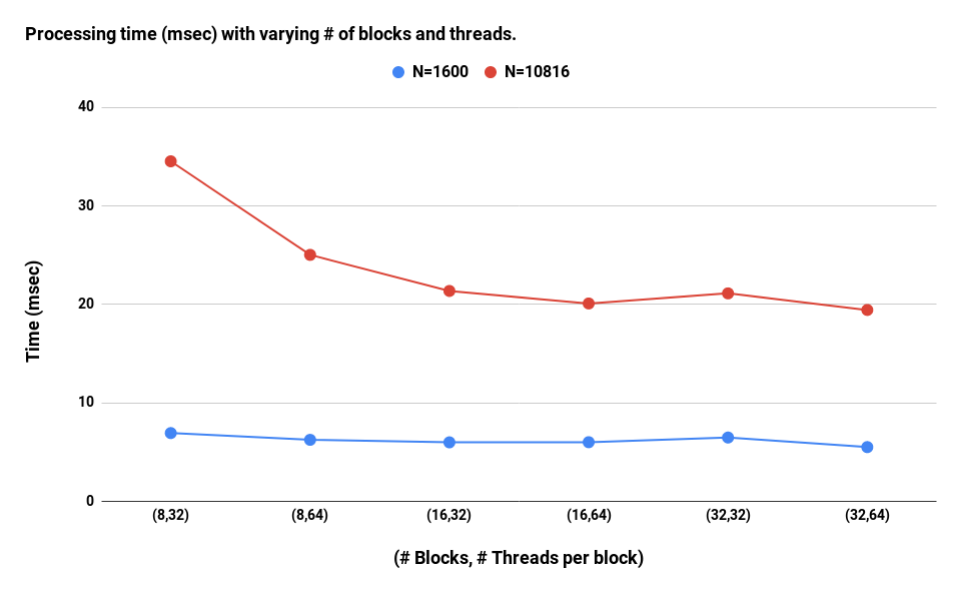
\includegraphics[scale=.40]{proctime.png}
        \caption{\label{gpu_scaling} Processing time in msec for varying number of blocks and number of threads per block on a GPU for matrix sizes 1600 and 10816.} 
	\end{figure}
\end{center}

\subsection{Potential Coupling}


    All the major operations of CG such as matmul, dot product, vector additions/subtractions can be replaced with other libraries like Metis, MKL etc. \\ 
    Advanced Decomposition (Metis): As discussed in section 3.1.2, one possible way to parallelize the CG code is to decompose the Poisson grid in a way that the stencil operation (matmul) can be applied to individual domains. The decomposition is not direct as boundaries have to be either copied or shared among neighbouring domains. For this purpose, Metis library can be used. 
    
    \\
    Solver Libraries (MKL): MKL library can surely be used for CG. It offers different BLAS Levels for different type of operations. Level 1 is for vector-vector operations which can be used for vector additions/subtraction and dot product functions in CG. Level 2 is for matrix-vector operations which can be used for the matmul operation. MKL also provides functions for Sparse Matrix vector multiplication (required for Poisson matrix) with different types of compression techniques like Compressed Sparse Row (CSR), Coordinate List (COO). However, parallelizing sparse matrix operations is not simple as the accesses of the elements are not uniform in every row. The index vectors (different for different compression formats) are to be used to index into the matrix which is not uniform. Also, stencil operation is more efficient than storing in Sparse format as stencil operaton is eliminating the need for storing any matrix. 
    
    \\
    PETSc, Trilinios and Boost: PETSc, Trilinios and Boost libraries can also be used to implement CG. PETSc and Trilonios use the ideas of BLAS discussed above. PETSc supports multithreading. Boost also provides support for linear algebra operations. All support sparse matrix representation. 
    
    \\
    Parallel IO Libraries (HDF5): Referring to the parallelization technique proposed in section 3, on stencil operation using MPI, it will be useful to use a parallel IO library, like HDF5, along with MPI so that the overhead of decomposing the matrix can be avoided. Every cores can perform the stencil operation independent of the neighbouring cores and hence, avoiding the communication overhead. 
    
    \\
    Accelerators: I used OpenACC framework to execute CG on GPU as discussed above. As mentioned, the main research work focuses on accelerating CG for discrete Poisson problem, using FPGAs.
    \\
    \\
    For future work, I would like to use MPI and Parallel IO Libraries for parallelization on CPUs and improve the performance of execution on GPUs by reducing the transfer of data between Host and Device. I believe that using MPI for stencil operation might improve the performance of Parallel CG as the communication between nodes is more efficient using MPI. 
    
\section{Discussion and Conclusions}

I chose to solve the discrete Poisson problem on Cartesian Grid. Initially, I investigated on the solver to be used. The performance of direct solvers ($LDL^T$) and iterative solvers (CG) was shown and it was clear that there was a considerable speedup of the iterative solver over the direct solver primarily due to the stencil operation in the iterative solver instead of the expensive matrix-vector multiplication (matmul) in the direct solver. \\
In order to identify the most expensive operations in CG, I profiled it to find that matmul (stencil operation) is the major bottleneck. I used OpenMP framework to parallelize the CG implementation and obtained good speedup. I further analyzed the performance by scaling the number of parallel cores. \\
Finally, I implemented CG using OpenACC framework to execute it on GPU. I could not show an improvement in the performance as I did not optimize it fully due to time constraints. \\

For future work, firstly, I would like to completely optimize the OpenACC implementation and execute it on a GPU. I expect to obtain a great speedup with proper data transfer optimizations. One interesting experiment to do would be to compare OpenMP implementation with MPI implementation to investigate which technique would be most efficient for CG. One can use parallel IO libraries for better performance.\\

I would like to mention about one of the upcoming memory technologies - compute enabled memories. Researchers are working on processing in memory or near memory computing. A lot of work on vertical 3D memories  \cite{inmemory}, compute-enabled SRAMs \cite{neuralcache}, can already be found in literature. I believe leveraging this technology would tremendously improve the performance of SIMD operations. \cite{neuralcache} shows how  vector-additions and vector multiplications can be accelerated using bit-serial SRAMs. In order to use these technologies, custom ASICs have to be built and certain modifications to the existing notion of the operations has to be done. For instance, if bit-serial vector additions are to be used, the bits of each element has to be stored along the columns of the SRAMs instead of the rows. Processing in-memory would greatly improve the performance as the latency due to transfer of data can be eliminated. 

\newpage
\begin{appendices}

\section{Acknowledgements}
I would like to acknowledge my advisor Dr. Pawan Kumar, IIIT-Hyderabad, India for guiding me to work on conjugate gradient solver for discrete poisson equation on different architectures. I acknowledge my course instructors Dr. Adam Lavely and Dr. Chirstopher Blanton for providing the necessary resources and helping me resolve certain issues related to the codes.
I would like to acknowledge my class mates, Chirag Satish and Amatur Rahman, for helping me fix some implementation errors and clarifying some doubts regarding strong and weak scaling.

\section{Code}

The OpenACC code  is publicly accessible on GitHub. URL: https://github.com/sahithi-rv/ProjectReport3.
One can do git clone https://github.com/sahithi-rv/ProjectReport3.git to obtain the code repository.

The codes and instructions for compilation for the serial direct and iterative solvers is available on GitHub at: https://github.com/sahithi-rv/ProjectReport1

The codes and instructions for compilation for the parallel iterative solver is available on GitHub at: https://github.com/sahithi-rv/ProjectReport2.

\subsection{File names and Descriptions}

\begin{itemize}
\item OpenACC Code directory - acc\_src.
\begin{itemize}
    \item cg3.c - OpenACC CG implementation
\end{itemize}
\end{itemize}

\subsection{Compile and Run Instructions}

\begin{itemize}
    \item ssh -l  username login.xsede.org
    \item gsissh bridges
    \item interact -gpu -n 10 -t 02:00:00
    \item module unload icc
    \item module load pgi/18.1
    \item module load cuda/8.0
    \item export PGI\_ACC\_TIME=1
    \item pgcc -acc -fast -Minfo=acc,ccff acc\_src/cg3.c
    \item to run the code:
    \begin{itemize}
        \item ./a.out test\_matrices/b10816 104 198
        \item ./a.out test\_matrices/b1600 40 82
        \item ./a.out test\_matrices/b1024 32 61
    \end{itemize}
\end{itemize}

I connected to the Bridges on Pittsburg Super Computer (br005) to obtain access to the GPU (gpu045) using the XSEDE credentials. 

\section{Poster - separate document}
The poster is attached along with the report.

\end{appendices}


\bibliographystyle{acm}
\bibliography{finalReport}

\end{spacing}

\end{document}

%%%%%%%%%%%%%%%%%%%%%%%%%%%%%%%%%%%%%%%%%%%%%%%%%%%%%%%%%%%%%}}
